\headletter{A}
s discussed in the Introduction Section, this Chapter provides a complete related work overview of the main relevant topics addressed in the Thesis. In particular, Section~\ref{sec:iot} contains a large reference on the IoT-related technologies that represented a source of inspiration or a basis for the Chapters that will follow. In Section~\ref{sec:semantic_web}, instead, the Semantic Web vision and its capabilities are outlined. Some applications will be described to exemplify.

Then, in Section~\ref{sec:siot_sepa}, the base of IoT semantic approach for interoperability developed at ARCES is explored. Almost all the work exposed in this Thesis lays on such approach, that enables dynamic responsiveness in semantic contexts.

\section{Internet of Things}
\label{sec:iot}

Electronics is everywhere: it is \textit{pervasive} \cite{saha2003pervasive} both in the spatial and conceptual meaning of the term. That is, sensors are dispatched in almost every environment, and measure almost every physical entity available contributing with their data to countless applications. Actuators, in a similar way, trigger changes within the environment, so that users can benefit from the effects. 

The IoT revolution \cite{gubbi2013internet, atzori2010internet} deeply impacted many sectors of everyday life: nowadays research and industry are proceeding towards the smartification of reality, including smart homes \cite{stojkoska2017review}, smart cities \cite{zanella2014internet, betis2018ieee}, smart health-care \cite{solanas2014smart, catarinucci2015iot, borelli2019habitat}, smart agriculture \cite{gondchawar2016iot, patil2016model} and so forth.

Listing all possible architectures employed in IoT applications is a task that is almost impossible, due to the huge variety of the topics that over the time have been concerned by the smartification process. As a reference, anyway, here follows a description at high level of some of them, mentioning in particular the ones that are relevant for the next Chapters. 

IoT, as we said, is a term that was coined by Kevin Ashton in 1999~\cite{ashton2009internet}. The vision, indeed, has been since then modified to be coherent with the current available technologies. Just consider that back at that time Internet access was possible, but not as common as it is today, available in almost every home. This is an interesting indicator of how different might have been the perspective.

Devices, before being connected to the Internet, were directly communicating with one another and therefore we had short distance and small environments. To this extent, a rich collection of protocols and standards were developed like the USB standard, dating back to 1996, and Bluetooth, whose first device was being sold in late 1999\footnote{\faBluetooth~\url{https://www.bluetooth.com/about-us/our-history/}}. The connectivity through the Internet, due to the limited bandwidth available for data transfer, was not yet ready to support online sensors and actuators and the exchange of their data. 

During the following years silicon production processes and studies on computer architectures considerably evolved, revealing the bases of modern IoT. First of all, it was possible to have CPUs with more calculation power in less space; secondly, broadband connection to the Internet became a reality, together with new mobile communication systems (3, 4, and now 5G). In addition, various wireless protocols like Wi-Fi, ZigBee, 6LoWPAN, LoRa became easily available \cite{al2017internet}. In some cases, e.g., LoRa and 6LoWPAN, they were designed with the explicit goal of enabling IoT technologies. As Mulligan states in \cite{mulligan20076lowpan}, \textit{``The concept was born from the idea that the Internet Protocol could and should be applied to even the smallest of devices''}.

Researches like \cite{samie2016iot, guth2018detailed} provide a complete discussion on the IoT background, covering the various design layers from calculation units to communication protocols and global architecture.

Such availability of new computation and communication instruments revealed itself to be a powerful trigger for the spreading of IoT, which was then interpreted as the solution to many complex important problems. Moreover, the variety of approaches exponentially increased along with the number of questions that were answered through IoT techniques. So, as a result, defining and realizing an IoT project eventually produced others ideas, in a positive and creative feedback loop similar to the ones in Figg.~\ref{fig:iot_diagram} (a) and (b), that are a synthesis of the one exposed by Jacobson et al.~\cite{jacobson2017there}. As it can be seen there the \textit{problem} definition derives from the \textit{evaluation} of a previous project; a \textit{technical analysis} follows, where the state of the art is analyzed, and choices are made: which is the best hardware platform, which are the most effective communication protocols for this application? How to, in general, \textit{design} the IoT solution? 

\begin{figure}[t!]
	\centering
    \begin{subfigure}[b]{0.4\textwidth}
    \centering
   	\smartdiagramset{uniform color list=white for 6 items,
   	uniform arrow color=true, text width=3cm, font=\sffamily}
	\smartdiagram[flow diagram]{Co-create, Ideate, Q \& A, Map to OSI,
	Prototype, Deploy}
	\caption{}
	\label{subfig:jacobson}
    \end{subfigure}
    \quad
    \begin{subfigure}[b]{0.4\textwidth}
    \centering
    \smartdiagramset{uniform color list=white for 5 items, 
    uniform arrow color=true, text width=4cm, font=\sffamily, 
    module y sep=2cm}
    \smartdiagram[flow diagram]{Ideas, Problems, Technical Analysis, 
    IoT Solution Design, Usage \& Evaluation}
	\caption{}
    \label{subfig:jacobson_sinthesis}
    \end{subfigure}
\caption{Typical problem solving workflow for IoT projects, as exposed by Jacobson et al.~\cite{jacobson2017there} (\ref{subfig:jacobson}), and in a higher level synthesis (\ref{subfig:jacobson_sinthesis}).}
\label{fig:iot_diagram}
\end{figure}

Although depicting a rather general approach to engineering problems, Fig.~\ref{fig:iot_diagram} fits in a very special way the IoT, hiding its main drawback. Every step in these two flow charts is developed independently from one project to the other. This, eventually, produces applications and systems that work on their own, that are connected to their network, but still are unable to interoperate. Such broken communication may happen at any level of ISO-OSI stack, that is the centre of IoT interoperability, as it is reported by Banerjee et al.~\cite{banerjee2017iot} and by Rayes et al.~\cite{rayes2017internet}:
\begin{description}
\item[Physical and DataLink Layer: ] two IoT systems will not be able to interact properly if it is not possible to share the physical communication mean and if there is no match in the how they perform direct contact. This includes the usage of legacy and/or constrained networks or devices requiring specific setups \cite{bormann2014terminology}. Example: system A communicates with USB protocol, system B with Bluetooth.

When layers 1 and 2 are not matching, device and service \textit{local discovery} is impossible, signifying that devices and systems cannot even be aware that other devices and systems are dispatched in the same environment.
\item[Network and Transport Layer: ] given that two IoT systems share the same Physical and DataLink layers, their remote connection is possible only if routing is also possible from one to the other, and if they agree on how to perform information exchange. For instance, a system exploiting UDP vs a system using TCP and targeting a very different audience.

Layer 3 and 4 match is necessary for \textit{remote discovery} and complex data share mechanisms \cite{bello2017network}. 

\item[Upper layers: ] are necessary when the setup gets more complex than mere communication of raw data. IoT systems exploiting upper layers share higher level information, which has to be interpreted in the very same way: from the character sequence choice to the content scheme used to format the data.

A relevant example, here, may be the interaction of two different entities when one produces JSON-formatted data, and the other expects XML. Or, similarly, when they both interact through JSON, but the former uses the tag \textit{\texttt{book}} to identify an instance of literary creation, and the latter as the action of making a reservation for a flight.
\end{description}

A sequence of choices is made for every IoT system within this stack. This builds up the concept of \textit{vertical silos}, which means that once that two developed applications are up and running, either the design choices are the same, either at some point information will get stuck and collaboration will not be possible. Studies on how to overcome this fragmented vertical reality were performed since the very beginning of IoT era, and resulted in an extremely rich literature \cite{mora2018collaborative, bandyopadhyay2011role}. Among the results, research provided over the years also
\begin{itemize}
\item New protocols like AMQP, MQTT, CoAP \cite{soni2017survey, yassein2016application}. In such context, devices are supposed to be able to use application layer protocols (i.e., they have enough memory and computational power to implement all the stack), and use a topic-based logic to exchange information. That is, interoperability is defined as an agreement on a topic taxonomy, and data is exchanged through a middleware that is able to implement communication on top of topic channels.
\item Translators from a protocol to the other, like presented in \cite{derhamy2017iot, palavras2018semibiot}, or from one hub to the other \cite{blackstock2014iot}. This means, in particular, that the communication between entities is mediated by a third entity designed to act as a gateway \cite{vivek2015enabling, aloi2016mobile}. This approach, in some cases, generated heavy critics because of gateways development complexity, and privacy issues \cite{zachariah2015internet};
\item Information level interoperability, which may be considered as a mixture of the two previous points, in addition with semantic techniques \cite{desai2015semantic, broring2018big, ganzha2018towards, antunes2018towards}. This approach will be largely explored in this Thesis: it requires applications and systems to organize their data according to standardized schemas (i.e., ontologies). 
\end{itemize}

Globally, anyway, what is clear is that there must be a level shared by all IoT projects and systems to make environments communicate to each other and to assure that, for the future, service update will not imply a complete and expensive redesign. 

It is worth saying also that the concepts of Cloud Computing before \cite{josep2010view}, and Fog Computing later \cite{bonomi2012fog}, were in the end pursuing that same idea of achieving full connection of information. In fact, Big Data \cite{oussous2018big} has been largely feeding from both of them but still, among its known drawbacks \cite{kaisler2013big, gudivada2015big}, the disorder and incoherence of information are probably the mostly well known.

The three points previously listed besides show that information interoperability is the key for breaking the silos, even more than protocol aspects (whose lifecycle brings them to evolve continuously following technological trends). As a matter of fact, even the new facet of IoT, i.e. the Web of Things (WoT) \cite{guinard2011internet, raggett2015web}, whilst calling for the uniform usage of the protocols of the web in the IoT, must face the problem of interpretation of resources.

In this Thesis, to achieve this shared access to information we exploit the capabilities of the Semantic Web  to describe data generated by machines in a machine understandable way \cite{berners2001semantic, shadbolt2006semantic}. The next Section will provide some general examples of it, while Section~\ref{sec:siot_sepa} will explain some tools necessary for an application of the Semantic Web to the Internet of Things world: the SPARQL Event Processing Architecture.

%\hl{kazmi2016overcoming, fantacci2014short, datta2016datatweet, The internet of things has a gateway problem, IoT interoperability: A hub-based approach, A mobile multi-technology gateway to enable IoT interoperability, IoT interoperability—On-demand and low latency transparent multiprotocol translator, User interoperability with heterogeneous IoT devices through transformation, The BIG IoT API-Semantically Enabling IoT Interoperability, Enabling IoT Platform Interoperability Using a Systematic Development Approach by Example, Interoperability in internet of things: Taxonomies and open challenges}

%\hl{Direct communication, low-range protocols; Constrained devices; Edge-Fog Computing; Cloud-Computing; Middleware IoT, MQTT, AMQP; Web of Things by Guinard; IFTTT and related apps; LoRa;}

\section{The Semantic Web}
\label{sec:semantic_web}

The possibility to freely interlink any piece of information and any service with all the others is to be considered over the time one of the reasons of the great success of the Internet. However, the idea that Web resources could be better organized is also quite old. Internet chaotic approach was heavily criticized as the Web reached its status of information and service provider. 

How to discover resources, how to perform requests, if no agreement is made on how contents are placed?

A first architectural answer to these questions was given in the research that introduced the REpresentational State Transfer (REST) pattern \cite{fielding2002principled} conducted in 2000 by Roy Fielding. The suggested approach provides a set of rules on how to organize systems whose information and services are web-based. Nowadays this is \textit{de facto} a standard, and contributed heavily to the development of actual standards like HTTP 1.1 \cite{fielding2014hypertext} and URI \cite{berners1998uniform}. Moreover, the IoT and the WoT were also influenced, and several architectures were proposed in litterature \cite{cheng2018lightweight, laine2012restful, guinard2011internet}.

Nevertheless, RESTful architecture and principles (and its constrained version, called CoRE\footnote{\faLink~\url{https://datatracker.ietf.org/wg/core/about/}}) do not provide a logical taxonomy to describe the reciprocal relationship between resources, excepted the request of a tree setup. Such logical meta-information is demanded to the standards introduced in the Semantic Web \cite{berners2001semantic, shadbolt2006semantic}, namely OWL\footnote{\faLink~\url{https://www.w3.org/TR/owl2-overview/}}, RDF\footnote{\faLink~\url{https://www.w3.org/TR/rdf11-mt/}}, RDFS\footnote{\faLink~\url{https://www.w3.org/TR/rdf-schema/}} and SPARQL Language\footnote{\faLink~\url{https://www.w3.org/TR/sparql11-overview/}}. Briefly, this can be summarized as it is explained in Fig.~\ref{fig:semantic_web_example}: the Semantic Web allows to organize resources, given as URIs, blank nodes, literals, in the form of triples \textit{subject-predicate-object}. The subject can be a URI or a blank node; the predicate must be a URI; and the object can be a URI or a blank node or a literal.

\begin{figure}
\begin{center}
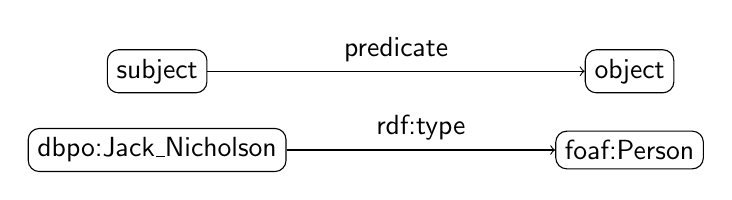
\begin{tikzpicture}
    \node[shape=rectangle, rounded corners, draw=black] (A) at (0,0) {\textsf{subject}};
    \node[shape=rectangle, rounded corners,draw=black] (B) at (6,0) {\textsf{object}};
    \node[shape=rectangle, rounded corners, draw=black] (C) at (0,-1) {\textsf{dbpo:Jack\_Nicholson}};
    \node[shape=rectangle, rounded corners,draw=black] (D) at (6,-1) {\textsf{foaf:Person}};

    \path [->] (A) edge node[midway, above] {\textsf{predicate}} (B);
    \path [->] (C) edge node[midway, above] {\textsf{rdf:type}} (D);
\end{tikzpicture}
\end{center}
\caption{An example of semantic triple storing the information that the resource URI related to Jack Nicholson makes reference to an entity of type Person, as it is defined in \ontoref{foaf} ontology.}
\label{fig:semantic_web_example}
\end{figure}

This network of triples, that can be extremely complex, results in a resource graph, which is also known as Knowledge Graph or Knowledge Base (KB). To make an example of Knowledge Graph it is worth citing DBpedia\footnote{\faLink~\url{https://wiki.dbpedia.org}}, which is \textit{a crowd-sourced community effort to extract structured content from the information created in various Wikimedia projects}, and is therefore open to all. It can be explored by using the SPARQL language, which we will largely use in the remaining of the Thesis.

To get an idea of how powerful is the setup provided by DBpedia, let us consider the following request: 
\begin{center}
\textit{Design a software that, by querying the Internet, will list an ``actor genealogy''.}
\end{center}

Starting from two actors, an ``actor genealogy'' is a sequence of triples \texttt{(actor1, actor2, film)} that allows in the minimum number $n$ of steps to connect the two actors through their films. For instance, trying to connect Jack Nicholson to Matt Damon should give, as possible result, a single triple connecting them through the well known 2006 film \textit{The Departed}. Instead, trying to connect Jack Nicholson and Julia Roberts results in two triples with George Clooney respectively in \textit{Batman\_1989\_series} and \textit{Ocean's Eleven}.

To address a problem like this, it is possible to avoid using DBpedia. Various services, on the web, provide APIs to list films, actors and their respective awards. However, here we will show that the semantic approach is definitely less expensive and more simple. For a non semantic approach, since we are interested in the shortest path from one actor to the other, a breadth first search is probably the easiest solution. Therefore, we expect to perform a sequence of requests to the web service, and list the films in which an actor starred, the other actors that were involved, iterating until there is a match for every actor in the sequence.

Instead, a semantic approach would simply search for patterns increasing in depth by 1 at each loop, as shown in the pattern in Listing~\ref{listing:actors}. Consequently, by using the semantic KB contained in DBpedia we will perform exactly $n$ requests for a $n$-step match, and we will not have to implement a breadth first search over a tree result.
\begin{lstlisting}[label=listing:actors, caption={SPARQL pattern example to solve the actor genealogy problem. Consider Table~\ref{tab:prefixes} for expanded prefixes.}]
# Direct match
SELECT ?film1 WHERE {
  ?film1 dbpo:starring <actor_in>, <actor_out>.
}

# One step match
SELECT ?film1 ?actor_1 ?film2 WHERE {
  ?film1 dbpo:starring <actor_in>, ?actor_1.
  ?film2 dbpo:starring ?actor_1, <actor_out>.
}
\end{lstlisting}

This example gives just a simple overview of how the Semantic Web can help. In general, however, we have that the graph in the KB is formatted according to specific ontologies, that represent a pattern for triple organization \cite{noy2004semantic}. In the \textit{List of Ontologies} Section it is possible to have a quick look on the ontologies that will be used in this Thesis. 

The ontology pattern is often considered as a bottleneck for the usage of Semantic Web. Ontologies, in many cases, are quite difficult to be understood and used: this creates a steep learning curve of the concepts and relationships expressed that, especially in a learning environment, can hinder the realization of applications. To address these obstacles, in the next Section some visualization techniques for the Semantic Web will be studied.

\subsection{Visualizing the Semantic Web}
\label{ssec:visualization}

This survey Section is based on a research work made at ARCES, aiming to create a better teaching-learning support for the students of the course \textit{Interoperability of Embedded Systems} held at the School of Engineering, University of Bologna. The following paragraphs are therefore inspired from the works\footnote{~\faCopyright~2018~IEEE.~Reprinted, with permission, from Antoniazzi, F., \& Viola, F. (2018, November). RDF Graph Visualization Tools: a Survey. In \textit{2018 23rd Conference of Open Innovations Association (FRUCT)} (pp. 25-36)} that were issued as a result of the research.

Accessing and understanding the content of a database is hardly ever a negligible task for programmers. When data is stored in a relational database, the views are obtained by transforming into a table the output of a query written in one of the various flavors of the SQL language. Smart-written queries on equally smart-built databases can efficiently perform a lot of calculations over data, as well as outline special and complex relationships even between apparently distant entries. Therefore the \textit{know-your-data} principle, typical of Data Mining and Big Data theory, is in fact a more general and solid base from which to start any data-related implementation, though implying sometimes great study effort from the developer in the initial phase of software creation \cite{han2011data}. It is, as a matter of fact, common knowledge that frequently programmers have to spend more time in organizing and reformatting their data more than in the actual programming logic.

The appearance of the Semantic Web in the panorama of information technology gave ways more than a simple new tool to explore the Web, but a new interpretation of the resources available on the Internet. Through the SPARQL language and the Resource Description Framework, the Internet network is considered as a whole a special database whose resources are interconnected in a labeled directed graph. The main idea of the Semantic Web, therefore, is to exploit the concepts of URI to bind resources through triple-based statements (i.e., the already mentioned subject-predicate-object triple). Any connection is in that fashion not a simple reference as hypertext linking is, but contains in addition the information given by the inner content of the resources. Then, according to W3C recommendations (see footnotes of Section \ref{sec:semantic_web}), the Semantic Web in the end takes the form of a graph, where both the contents and the statements contribute to the overall meaning. 

A few considerations are needed, however, when we start discussing about the possibility to store information in a semantic graph. In fact, some critical points are present, and have to be highlighted. First of all, as it is depicted in \cite{noy2005order}, without regulations, the semantic graph is doomed to chaos, i.e. to an unpredictable information taxonomy. The solution to this issue is the ontological description of knowledge, that consists in the formal definition of all the classes, relationships and statements that can be present in the graph. Once the programmers agree on the ontology, there is no uncertainty on how the data is organized. All the information needed to query the graph is stored in an OWL file, standing for Web Ontology Language. OWL is, according to W3C, a \textit{semantic markup language for publishing and sharing ontologies}, and has been widely used to define all sort of ontologies and vocabularies (which are smaller ontologies): an interesting repository, in this field of study, is the Linked Open Vocabularies website\footnote{\faLink~\url{https://lov.linkeddata.es/dataset/lov}} and, for the next Sections of this Thesis, the List of Ontologies.

A second critical point is connected to the dimension of the graph, which can be considerable not only when we are discussing about web-located knowledge bases like DBpedia \cite{lehmann2015dbpedia}, or the Internet itself, but also in smaller applications exploiting RDF and SPARQL. To make an example, let us perform the query of Listing~\ref{listing:lotr} to DBpedia.
\noindent
\begin{minipage}[c]{0.7\linewidth}
\begin{lstlisting}[caption={SPARQL query to all classes parent of the resource \texttt{dbpedia:The\_Lord\_of\_the\_Rings}},label={listing:lotr}]
SELECT (count(?o) as ?count) 
WHERE {
  dbpedia:The_Lord_of_the_Rings 
  	rdf:type ?o
}
\end{lstlisting}
\end{minipage} % no space if you would like to put them side by side
\begin{minipage}[c]{0.3\linewidth}
\noindent
\begin{center}
\faQrcode~\textsf{Query execution:}\\
\vspace*{0.2cm}
\qrcode{http://dbpedia.org/snorql/?query=SELECT+\%28count\%28\%3Fo\%29+as+\%3Fcount\%29+\%0D\%0AWHERE+\%7B\%0D\%0A++\%3AThe_Lord_of_the_Rings+\%0D\%0A++\%09rdf\%3Atype+\%3Fo\%0D\%0A\%7D}
\\
\tiny{\textsf{Last visited: 15/10/2019}}
\end{center}
\end{minipage}
\noindent
\begin{minipage}[c]{0.7\linewidth}
\begin{lstlisting}[caption={SPARQL query to every link (except \texttt{rdf:type}) with \texttt{dpbedia:The\_Lord\_of\_the\_Rings} as origin, and the destination's class},label={listing:lotr2}]
SELECT ?p (count(?t) as ?count) 
WHERE {
  dbpedia:The_Lord_of_the_Rings ?p ?o.
  ?o rdf:type ?t
  FILTER (?p != rdf:type)
}
\end{lstlisting}
\end{minipage} % no space if you would like to put them side by side
\begin{minipage}[c]{0.3\linewidth}
\noindent
\begin{center}
\faQrcode~\textsf{Query execution:}\\
\vspace*{0.2cm}
\qrcode{http://dbpedia.org/snorql/?query=SELECT+\%3Fp+\%28count\%28\%3Ft\%29+as+\%3Fcount\%29+\%0D\%0AWHERE+\%7B\%0D\%0A++\%3AThe_Lord_of_the_Rings+\%3Fp+\%3Fo.\%0D\%0A++\%3Fo+rdf\%3Atype+\%3Ft\%0D\%0A++FILTER+\%28\%3Fp+\%21\%3D+rdf\%3Atype\%29\%0D\%0A\%7D}
\\
\tiny{\textsf{Last visited: 15/10/2019}}
\end{center}
\end{minipage}

The output of the query, which is a simple request to count all the classes that ``The Lord of the Rings'' resource belongs to, is equal to 25. Clearly, far from a naive and optimistic expectation of a few outputs similar to \texttt{:Book}, \texttt{:Novel} and so on. Listing the actual values consequently results in a 25-rows table that outlines the evidence of the hidden complexity in the results analysis, even in simple situations. The complexity grows considerably if we proceed querying on the following level (Listing~\ref{listing:lotr2}).

The query available in Listing \ref{listing:lotr2} with the variable \texttt{?count} outputs the number of links of type \texttt{?p} outgoing from the resource \texttt{dbpedia:The\_Lord\_of\_the\_Rings}, except from \texttt{rdf:type} links, that can be viewed by performing the query in Listing \ref{listing:lotr}.

The direct outcome after running the queries in the Listings \ref{listing:lotr} and \ref{listing:lotr2} is given by the possibility to observe the available variability of results and to look for their meanings. The output of those simple SPARQL queries highlights, for instance, that the ``Lord of the Rings'' resource is individual of at least 25 classes which we expect to have a specific meaning and a description of their own. Going further with the latter query, moreover, the number of elements connected to the resource is even more increasing, both as connectivity spread, and in diversity of ontological classes involved. In general the description of all those resources can be as pragmatic as an algorithm, or philosophical, or mathematical. However, it is clear that without the Semantic Web it would be hardly achievable to obtain such a multi-layered description of a resource, apart from using natural language. In fact, when it comes to exploit the tools of Semantic Web, a frequent feeling is that it is not possible to reuse previously available data, because it would imply to understand completely all the resources, all the classes, and all the ontologies that are standing behind. According to \cite{920602}, expressiveness, in this situation, is a bottleneck for Semantic Web.

This is where visualization tools for the semantic graph come to help: they provide a step by step approach to the knowledge base that, together with filtering techniques, and the possibility to see the contents, are useful to go through the relevant concepts.

\subsubsection{\textsf{Possible visualizations}}

As we said previously, the most frequent way to produce a view of a database is the tabular representation. This is a possible solution also for queries made in SPARQL language to RDF triple stores like Blazegraph, Fuseki and Virtuoso. The view of a SPARQL \texttt{SELECT} is a direct consequence of the number of variables concerned by the inquire: i.e., the number of variables in the \texttt{SELECT} clause is the same as the number of columns contained in the results. To be more precise, to obtain the column number either (i) it is necessary to count the variables queued after the \texttt{SELECT} keyword, like in listings \ref{listing:lotr} and \ref{listing:lotr2}; or (ii), variables have to be obtained from the \texttt{WHERE} clause, as in the \texttt{SELECT * WHERE \{...\}} case.

The drawbacks with table views are, unfortunately, already quite visible when the number of rows reaches as little as few dozen entries. Aside from the fact that there is not a group view of the overall query result, the table often is required to contain more than one row for the same conceptual entity. This happens for instance when a resource is connected to another via more than one predicate, or when it is connected to different objects, through the same predicate.

In such situations, the result table can contain not only plenty of lines with the same meaning disturbing the overall understanding of the query output, but also, as already said, a high number of columns. Moreover, some entries in the table can also be empty, as an effect of \texttt{OPTIONAL} statements in the query. Detecting particular cases, in sparse and large tables, becomes a time-consuming and error-prone task in those situations. On the other hand, a few workarounds are available in \texttt{SPARQL} language to crunch into a single line the occurrence of multiple table lines for a single concept, but they usually imply slowing down the performances, and have the effect to concatenate the values into strings. That is, we lose the possibility to check if they are represented as IRIs, literals, or blank nodes.

The multi-table approach is a graph visualization technique that tries to address the problem of having limited control over the complete data table. Let's consider a query selecting all triples in the RDF store: \texttt{SELECT * WHERE \{?a ?b ?c\}}, and let's suppose that in the store only 5 distinct resources might correspond to the \texttt{?b} variable. With this background a full-table approach would return an $n=3$ column table, where $n$ is the number of variables. Instead a multi-table approach would outcome with 5 smaller tables, one for each one of the \texttt{?b} resources, each of them built up of $n-1=2$ columns. An interesting work about the complexity of translation from SPARQL to other languages, included table view, was provided by Chebotko et al. in \cite{chebotko2007storing}: among all the contributions, this paper perfectly shows the complexity of a multi-table approach.

Finally, last but not least, the RDF knowledge base representation can be performed through a labeled graph visualization. Although the RDF concept is defined for directed graphs, in most of the cases the label is sufficient to get at view time the direction of the connection. This allows the usage of algorithms for undirected graphs. Nevertheless, the drawbacks of this approach are also related to the knowledge base dimension, as the understanding of contents is tightly bound to the possibility of identify paths and node types easily and effectively.

\subsubsection{\textsf{Graph drawing algorithms}}

There is a complex relationship between the domain of the semantic application, the tool that is being used, and the algorithm that is implemented to visualize the graph. To make an example, let's consider a knowledge base in which information about some people is stored. If the application working on the knowledge base is not interested in literal terms, the sight of the graph would be effectively simplified and clearified by just removing all the links towards literal terms, e.g. names, surnames and birth dates. 

In other RDF triple stores more than one unique ontology may have been used to define resources, exploiting for instance simultaneously the \ontoref{foaf} ontology and the Dublin-Core ontology \ontoref{dc}. If an application is interested only in the \ontoref{foaf}-related connections, and in a small part of the DC's, there would be no use in trying to represent everything.

A full description of all the algorithms available for graph drawing is out of the scope of this Thesis. In this Section, nevertheless, a brief overview of a few works available in literature is given, before proceeding in the next paragraph to the analysis of the tools.

A complete theoretical overview of the main algorithm logic available to draw graphs is given by Kobourov in \cite{kobourov2012spring}. Spring algorithms and their variations for instance are explained: they usually aim to reproduce an aesthetically pleasant view, even if their best performance is obtained in most of the cases when the graph has less than 40 vertices. However, as it has been said, the semantic graph is definitely a large graph, or very large, and for this reason it demands particular approaches that imply multiple scale algorithms. Nodes organization is not necessarily done on a plane: possible alternatives are to dispose them on a sphere or other geometrical objects. In \cite{viola2018interactive} more than one plane is used, which can be a technique also to represent the evolution of data over time. How to show in an effective way dynamic evolution of contents in a graph is also the topic of survey \cite{beck2017taxonomy} by Beck et al.

\noindent
\begin{minipage}[c]{0.7\linewidth}
\begin{lstlisting}[caption={SPARQL \texttt{CONSTRUCT} that identifies in DBpedia the Fantasy-genre books written between 1900 and 2018 having more than 200 pages.},label={listing:fantasy}]
CONSTRUCT {
  ?book rdf:type dbpo:Book; 
    dbpo:literaryGenre :Fantasy_novel;
    dbpo:author ?author;
    dbpo:releaseDate ?date;
    rdfs:comment ?comment;
    rdfs:label ?label;
    dbpo:numberOfPages ?num;
    foaf:isPrimaryTopicOf ?topic.
  ?author rdf:type foaf:Person 
}
WHERE {
  ?book rdf:type dbpo:Book;
    dbpo:literaryGenre :Fantasy_novel;
    dbpo:author ?author.
  ?author rdf:type foaf:Person.
  ?book rdfs:comment ?comment;
    rdfs:label ?label;
    dbpo:numberOfPages ?num;
    foaf:isPrimaryTopicOf ?topic.
  FILTER langMatches(lang(?label), "EN")
  FILTER langMatches(lang(?comment), "EN")
  FILTER (isIRI(?author))
  FILTER (xsd:integer(?num) > 200)
  OPTIONAL {
    ?book dbpo:releaseDate ?date .
    FILTER (?date > 1900)
    FILTER (?date < 2018)
    FILTER (isLiteral(?date))
    FILTER (datatype(?date) = xsd:integer)
  }
} 
\end{lstlisting}
\end{minipage} % no space if you would like to put them side by side
\begin{minipage}[c]{0.3\linewidth}
\noindent
\begin{center}
\faQrcode~\textsf{Query execution:}\\
\vspace*{0.2cm}
\qrcode{https://bit.ly/2OUYTnX}
\\
\tiny{\textsf{Last visited: 15/10/2019}}
\end{center}
\end{minipage}
\subsubsection{\textsf{Graph visualization tools}}

Hereby a detailed analysis of the main tools for the visualization of RDF knowledge bases and ontologies is proposed. We focus on the tools providing a graph visualization of RDF statements. The tools presented in this Section are reported in alphabetical order.
\begin{description}[wide, labelindent=0pt]
\item[CytoScape] is a tool for network data integration, analysis and visualization. Support to Semantic Web technologies is provided by a set of extensions hosted on CytoScape's App Store, such as General SPARQL,  SemScape and Vital AI Graph Visualization \cite{shannon2003cytoscape}.
General SPARQL allows to navigate semantic web KBs through an extensible set of pre-defined queries. The plugin is pre-configured to retrieve and visualize data from public endpoints (e.g., Reactome, Uniprot, HGNC, NCBI Taxonomy, Chembl). SemScape supports the interaction with remote SPARQL endpoints by means of SPARQL queries. In this way, CytoScape can be employed to visualize the results of a query. Vital AI Graph Visualization is not limited to semantic databases, but provides access also to SQL and NoSQL databases as well as Apache Hadoop instances. To the best of authors' knowledge, this tool only allows the visualization of data compatible with the BioPAX format.
\item[Fenfire] was a tool for the visualization and editing of RDF graphs aimed at an interactive exploration of the graph \cite{hastrup2008browsing}. Authors face the problem of scalability by
limiting the exploration of the graph to one thing at a time. The visualization in facts, diplays only one central node and its surroundings. The central node, at the beginning of the exploration is selected exploiting the \texttt{foaf:primaryTopic} property (if present), otherwise is selected by the user. The nodes surrounding the central one (named \textit{focus}) are placed on the plane according to a simple strategy: on the left, all the nodes being subjects of the statements linking to the focus. On the right, those being objects of the statements. Development of Fenfire stopped in 2008.
\item[Gephi] is a very powerful tool designed to represent not only semantic graphs, but every kind of graph or network \cite{bastian2009gephi}. Support to RDF graphs is provided by two external plugins, VirtuosoImporter and SemanticWebImport (this one developed by INRIA). Gephi is able to retrieve data from SPARQL endpoints (through REST calls) as well as to load RDF files. Gephi supports filtering the KB through SPARQL queries. The look of the graph visualized by Gephi is fully customizable, in terms of colors and layouts; moreover the tool supports grouping similar nodes and this helps achieving better results when dealing with very complex graphs. As regard exporting the graph, Gephi is the tool that supports the highest number of file formats for exporting the graph. Among these, it is worth mentioning \texttt{csv}, \texttt{pdf} and \texttt{svg}.
\begin{figure}[!t]
    \centering
    \begin{subfigure}[b]{\textwidth}
        \includegraphics[width=\textwidth]{gephi1.png}
        \caption{The Figure is the output of Gephi's \texttt{CONSTRUCT} in Listing~\ref{listing:fantasy} to DBpedia. According to its logger, the triples represented in this graph are 6529.}
        \label{fig:fullgraph_gephi}
    \end{subfigure}

    \begin{subfigure}[b]{\textwidth}
    \centering
        \includegraphics[width=0.8\textwidth]{gephi2.png}
        \caption{With Gephi some nodes can be highlighted, to help the user to go through the knowledge base. When the number of edges and nodes is high, however, it's not easy to outline the information. The nodes in red are related to L. Alexander's novel ``The Black Cauldron''.}
        \label{fig:blackcauldron}
    \end{subfigure}
    \caption{Gephi~\cite{bastian2009gephi} output example.}
    \label{fig:gephi_figs}
\end{figure}

In Figure \ref{fig:fullgraph_gephi} we can see a view of the graph that Gephi is able to retrieve from DBpedia by using the SPARQL \texttt{CONSTRUCT} available in Listing \ref{listing:fantasy}. The tool performs the representation very quickly, and implements various possible algorithms to build the graph. Unfortunately, as it can be seen, it is quite difficult to get the overall idea of the composition. Although there is the possibility to add the labels of nodes and edges, the output is not reader-friendly, and the research in it is a rather impossible task. A practical example can be observed also in Figure \ref{fig:blackcauldron}, where we highlighted the nodes related to the novel ``The Black Cauldron'' by L. Alexander. Eventually, a number of statistical functions can be applied to the network, like the \textit{Network Diameter}, the \textit{Density} and the \textit{Average Path Lenght}: the only problem is that they have, as for the Authors' knowledge, very limited use when applied to a Semantic Graph.

\item[Glow] is a visualization plugin for the ontology editor Prot\'eg\'e \cite{hop2012using}. Force-directed, Node-link tree and Inverted radial tree are the three layout algorithms provided by GLOW. The items are arranged automatically with every layout, and cannot be moved. The tool is able to represent a set of ontologies and optionally their individuals. To the best of authors' knowledge, this tool is not developed anymore. No information about the license could be found. 

\item[IsaViz] is a 2.5D tool for the visualization of RDF graphs originally developed by E.~Pietriga (INRIA) in collaboration with Xerox Research Centre Europe \cite{pietriga2003isaviz}. IsaViz, as the name suggests, is based on GraphViz~\cite{ellson2001graphviz} and allows importing and exporting from/to RDF/XML, Notation 3 and N-Triple files. The result of the visualization can be also exported as a \texttt{png} or \texttt{svg} file. In the \textit{Graph view} it is possible to select resources and access a textual list of properties (this view is named \textit{Property Browser}). A third view is named \textit{Radar} and presents an overview of the graph, since the graph view may contain only a portion of it. Finally, it is worth mentioning the search tool provided by IsaViz, whose results are highlighted one by one in the graph view. Unfortunately, the last development version of this tool dates back to 2007.

\item[Jambalaya] is a Prot\'eg\'e plugin for the visualization of ontologies \cite{storey2002jambalaya}. Jambalaya is characterized by the integration of the SHriMP (Simple Hierarchical Multi-Per\-spec\-tive) \cite{storey2001shrimp} visualization technique, designed to improve the user experience in browsing, exploring, modelling and interacting with complex information spaces. This technique, originally born to help programmers understanding software, was applied to Prot\'eg\'e to build a powerful visualization of classes and relationships. 
The tool proposes a nested graph view and the nested interchangeable views. Nesting is used to represent the sub-class relationships among classes as well as the link between classes and their instances (different colors allow to distinguish between classes and instances).
Jambalaya also provides an easy way to search for items in the ontology. Despite being an interesting tool developed with support from the National Center for Biomedical Ontology~(NCBO), Jambalaya is not developed anymore.

\item[LOD Live] is a web-based tool for the incremental navigation of Linked Data available on a selected SPARQL Endpoint (e.g., DBpedia) \cite{camarda2012lodlive}. Endpoints can be configured through a JSON map of their parameters, similarly to what happens in Tarsier~\cite{viola2018interactive}. The purpose of this tool is to demonstrate that the powerful Semantic Web standards are also easy to understand; the aim is to foster the spread of Big Data. Every resource drawn by LOD Live is surrounded by a set of symbols representing different kinds of relationship (e.g., direct relations, group of direct relations, inverse relations and group of inverse relations). The incremental navigation, joined to the ability of the tool to group properties allows to draw a very clean graph. No support for statistics or advanced filtering (e.g., based on SPARQL) is provided. To the best of our knowledge, directly exporting the graph is not possible. In Figure \ref{fig:lodlive} it is shown how LOD Live performs a similar task as the one in Figure \ref{fig:blackcauldron}: exploring data is easier, but there is no way to perform requests like the one in Listing \ref{listing:fantasy}.
\begin{figure}
\centering
\includegraphics[scale=0.3]{lodlive.png}
\caption{To use LOD Live~\cite{camarda2012lodlive} a resource must be fixed. Then, the knowledge related to the resource can be expanded as shown. Like in Figure \ref{fig:blackcauldron}, the example here is based also on L. Alexander's novel ``The Black Cauldron''.}
\label{fig:lodlive}
\end{figure}

\item[Ontograf] is one of the visualization tools provided by the famous ontology editor Prot\'eg\'e \cite{falconer2010ontograf}. The tool allows to build a custom visualization of the ontologies loaded in Prot\'eg\'e by iteratively enabling or disabling the desired classes. Ontograf proposes a grid layout (with classes sorted in alphabetical order), a spring layout and a (vertical or horizontal) tree layout. Individuals of a class can be visualized in its tooltip, but this is uncomfortable when dealing with a high number of assertional statements. Ontograf allows to export the visualized graph as a png, jpeg, gif or dot file. This tool exploits the layout library provided by Jambalaya.
\begin{figure}
    \centering
    \includegraphics[width=.75\textwidth]{ontograf.png}
    \caption{A portion of the DBpedia ontology visualized in Ontograf~\cite{falconer2010ontograf}.}
    \label{fig:ontograf}
\end{figure}
Fig.~\ref{fig:ontograf} shows a graph created with OntoGraf using the DBpedia ontology. Classes \texttt{work} and \texttt{written work} were initially selected. Then, a double click on the latter allowed to expand it and visualize all the subclasses (solid blue line), and all the classes linked to it by means of an object property (dashed lines). The last version of Ontograf dates back to April 2010, but is still included in the last stable version of Prot\'eg\'e\footnote{\faLink~\url{https://protege.stanford.edu/}}~(the 5.5.0, as of August 2019). The tool is useful to select and visualize (a small number of) classes from the ontologies loaded in Prot\'eg\'e and the existing relationships.

\item[OntoSphere] is one of the two tools (the other is Tarsier~\cite{viola2018interactive}) that proposes a three-dimensional visualization of the graph \cite{bosca2005ontosphere}. The rationale behind OntoSphere is that exploiting a 3D space it is possible to better arrange items. Moreover, the 3D visualization is quite natural for humans and the exploration can then be more intuitive. Colors allow to easily convey information about the different nature of represented items. OntoSphere is aimed at representing both terminological and assertional statements. Four scene types are proposed to fulfill different requirements. The \texttt{RootFocus} scene shows all the concepts and their relationships on a sphere. The \texttt{TreeFocus} scene draws the tree originating from a concept, while the \texttt{ConceptFocus} scene proposes a view containing all the items linked to a concept. The tool is aimed at domain experts dealing with the development and review of ontologies, as well as novice users that wants to understand the represented data and the links among concepts. OntoSphere is a standalone applications, but can also be run inside Prot\'eg\'e and Eclipse. The last version on the source code repository is dated 2008, so the development stopped ten years ago.

\item[OWLViz] is a plugin for Prot\'eg\'e that enables the incremental visualization of the classes in the class hierarchy \cite{horridge2010owlviz}. As the name suggests, this tool, like IsaViz, is based on the famous library GraphViz developed by the AT\&T and allows exporting the visualized graph as \texttt{png}, \texttt{jpeg} and \texttt{svg}. Through OWLViz is easy to visualize classes and \texttt{is-a} relationships. OWLViz is not developed anymore, but is still included in the last version of Prot\'eg\'e (August 2019).

\item[Paged Graph Visualization (PGV)] is a Java software for the visualization of RDF graphs \cite{deligiannidis2007rdf}. It is based on \cite{janik2005brahms}, a high performance RDF storage. With PGV, the exploration starts from a point of interest and then incrementally includes more data. Such point of interest can be selected interactively from a list or using a complex SPARQL query. Then, it is drawn in the center of the graph using the color green, and its direct neighbors are shown as blue rectangles placed around it. Literals on the other hand, are represented with the white color. The user is able to explore nodes by double-clicking on them: explored nodes are then displayed in green, while edges connecting explored nodes are depicted in red. Deligiannidis et al.~\cite{deligiannidis2007rdf} declare that the tool's strength relies in helping the user willing to explore data without knowing the exact information and graph patterns he is looking for, while in other situation a standard visualizer could be more appropriate. This tool seems to be not developed anymore.

\item[RelFinder] is a web tool developed using Adobe Flex and can be tried using the web instance linked in the homepage of the project (configured to access DBpedia) \cite{heim2009}. RelFinder differs from the other tools proposed in this survey, since it is aimed at visualizing all the paths connecting two resources. So, its purpose is to answer a very specific question, rather than providing a tool for the free exploration of the knowledge base. The tool supports filtering to increase or reduce the number of relationships shown simultaneously. It also implements a smart drawing algorithm to reduce overlapping and the user is allowed to move and pin items. To the best of authors' knowledge, this tool is not actively developed but the online instance is still available for tests on the DBpedia endpoint. Fig.~\ref{fig:relfinder} reports an example of this application where all the paths between two DBpedia resources, i.e, ``JRR Tolkien'' and ``The Lord of the Rings'', are shown. 
\begin{figure}[!t]
    \centering
    \includegraphics[width=0.8\textwidth]{relfinder_short.png}
    \caption{RelFinder view of the paths from ``JRR Tolkien'' to ``The Lord of the Rings''.}
    \label{fig:relfinder}
\end{figure}

\item[Tarsier] is a tool developed by ARCES research group. It is a software for the interactive exploration of an RDF graph in a three-dimensional space, aimed at the visualization of small and medium-sized knowledge bases. The main contribution of the tool is the introduction of the metaphor of semantic planes that group RDF terms sharing a common concept. The purpose of the tool is threefold: 1) Tarsier can be used as a support for didactic (e.g., to help newcomers to deal with Semantic Web technologies); 2) It is useful to figure out the nature of a new KB for developers (i.e., activity known as ``sensemaking'' \cite{motta2011novel}) ; 3) It allows debugging of semantic knowledge bases.

Tarsier retrieves data from SPARQL endpoints. The initial knowledge base can be determined through a SPARQL Contruct query: this pre-filtering stage allows to efficiently interact also with very large knowledge bases (e.g., DBpedia, that contains more than 6.6M entities). Tarsier proposes a classification of all the RDF terms among classes, resources, blank nodes, literals, object and datatype properties. This grouping is exploited by Tarsier's web interface to provide a set of controls for advanced filtering: through them, the user is allowed to toggle visibility of items or to move them across semantic planes.  

An example of Tarsier is shown in Figg.~\ref{fig:tarsier} and~\ref{fig:tarsier-filter}. Tarsier was set up to retrieve data from DBpedia, and in particular to extract all the fantasy books published between 1900 and 2018 and their authors. While Fig.~\ref{fig:tarsier} shows the unfiltered knowledge base, in Fig.~\ref{fig:tarsier-filter} is shown one of the peculiarities of Tarsier: the semantic planes. Two semantic planes were created over the main knowledge base to extract respectively books and one of the authors, i.e., Marion Zimmer Bradley. In this way, it is easy to notice how this instance of the class \texttt{foaf:Person} is linked with the graph.
\begin{figure}[!t]
    \begin{subfigure}[b]{0.5\textwidth}
    \centering
        \includegraphics[width=\textwidth]{tarsier.png}
        \caption{Tarsier showing the graph of all the fantasy books published from 1900 to 2018 and their authors. This subgraph is retrieved from DBpedia.}
        \label{fig:tarsier}
    \end{subfigure}
    \hspace{0.5cm}
    \begin{subfigure}[b]{0.5\textwidth}
    \centering
        \includegraphics[width=\textwidth]{tarsier-filtered.png}
	\caption{Tarsier showing two semantic planes over the main knowledge base: one showing books, the other (the topmost) showing the author Marion Zimmer Bradley.}
    \label{fig:tarsier-filter}
    \end{subfigure}
    \caption{Tarsier~\cite{viola2018interactive} user interface.}
    \label{fig:tarsier_figs}
\end{figure}

\item[TGVizTab] is yet another visualization plugin for the ontology editor Prot\'eg\'e \cite{alani2003tgviztab}. It is designed to be lightweight and support both T-Boxes and A-Boxes visualization, and it relies on TouchGraph, an open source Java environment aimed at creating and navigating network graphs in an interactive way. The tool supports exporting the graph in an XML file, to be loaded in other TouchGraph applications. The graph is drawn using the spring layout: similar nodes are drawn close to each other. TGVizTab, like other tools (e.g., Fenfire), asks the user to select a focal node among classes and instances to generate the graph. Then, the user is able to further modify the graph by right-clicking on the represented nodes: in this way the so-called \textit{Node Menu} is shown, containing four options (i.e., expand, collapse, hide, view). Then TGVizTab allows to incrementally build the desired visualization.

\item[VOWL (Visual OWL)] is available as a web-based tool (WebVOWL~\cite{WebVOWL, lohmann2016visualizing}), a plugin for Prot\'eg\'e (Prot\'eg\'eVOWL~\cite{ProtegeVOWL}), a tool able to directly interact with Linked Data endpoints (LD-VOWL~\cite{weise2016ld}), and as a visual query language tool (QueryVOWL~\cite{haag2015queryvowl}). Here we will refer to the web based version, WebVOWL. As the name suggests, software in the VOWL toolkit are designed to graphically represent ontologies. They propose a force-directed graph layout. The basic representation rules adpoted by VOWL consists in:

\begin{itemize}
    \item Classes are depicted using circles where the color depends on the type: light blue for OWL classes, purple for RDFS classes, dark blue for those imported by other ontologies, gray for deprecated classes. 
    \item OWL object and datatype properties are represented with black solid lines with, respectively, light blue and green labels, while RDFS properties have purple labels.
    \item Relationships \texttt{subClassOf} are depicted with a dashed line.
\end{itemize}

The graph drawn by VOWL can be exported as an \texttt{svg} image or as a \texttt{json} file. A click on a node or edge allows visualizing the associated metadata and statistics. Statistics also report the number of individuals of the selected class, but unfortunately this is the only information about individual that is possible to obtain using VOWL. As regards filtering, VOWL provides a basic support to filters that allows to show/hide object/datatype properties, solitary classes, class disjointness and set operators.

VOWL is actively developed and an online instance is available. As the tool is designed for ontologies, importing the output of the \texttt{CONSTRUCT} in Listing \ref{listing:fantasy} results in representing only the two \texttt{rdf:type} relationships. The other tools are still being developed and at the moment do not allow to perform a customized request to DBpedia.
\end{description}

\subsubsection{\textsf{Overall considerations on graph visualization}}
Table~\ref{tab:summary} summarizes the main features of the analyzed software. Columns of the table are:

\begin{itemize}
  \item \textbf{Software} -- reports the name of the software;
  \item \textbf{T-Boxes} -- this column tells if the tool supports the visualization of terminological statements;
  \item \textbf{A-Boxes} -- this column shows if the tool supports the visualization of assertional statements (and can then be used to explore a knowledge base, rather than just ontologies);
  \item \textbf{Statistics} -- a boolean field showing if the tool provides or not statistics on the visualized data;
  \item \textbf{Filtering} -- filtering allows to show/hide elements in the visualization according to a set of user-defined criteria. Filtering can be implemented in very different ways (e.g., SPARQL queries, or UI controls to select classes, just to name a few). This column indicates whether the related tool provides at least one filtering mechanism.
  \item \textbf{Editing} -- This Thesis surveys visualization tools for semantic data, but some of them also offer editing functionalities. This column states whether or not the related tool supports the manipulation of the ontology/knowledge base;
  \item \textbf{Standalone} -- Many of the surveyed tools were born as plugins for the ontology editor Prot\'eg\'e. Other can be run as standalone software. This column tells if the related software is embedded in other tools or is a standalone application. 
  \item \textbf{Plugin} -- Not all the presented tools were born to visualize semantic knowledge bases. Then, some of them need additional plugins to achieve this task.
  \item \textbf{Domain} -- This column contains the specific domain (if any) where the related application can be applied.
  \item \textbf{Reference} -- This column reports the reference number of the paper(s) describing the tool.
\end{itemize}

Plus, additionally, other information about the entities that started the development of the tool, the license and the current status of the project.

\begin{sidewaystable}[t]
\centering \footnotesize
\caption{Summary of the features of the tools for the visualization of semantic knowledge bases. Legend: \faCheck = yes, \faTimes = no, \faExclamation = partial, \faCheckSquareO = multiple options available, \faQuestion = unknown, \faMinus = Not applicable}
\label{tab:summary}
\begin{tabular}{lcccccccc|p{5.5cm}ccp{1.2cm}}
\toprule
\textbf{Software} & \rotatebox{90}{\textbf{T-Boxes}} & \rotatebox{90}{\textbf{A-Boxes}} & \rotatebox{90}{\textbf{Statistics}} & \rotatebox{90}{\textbf{Filtering}} & \rotatebox{90}{\textbf{Editing}} & \rotatebox{90}{\textbf{Standalone}} & \rotatebox{90}{\textbf{Plugin}} & \rotatebox{90}{\textbf{Domain}} & \textbf{Developed} & \rotatebox{90}{\textbf{License}} & \rotatebox{90}{\textbf{Active}} & \rotatebox{90}{\textbf{Reference}} \\
\midrule

CytoScape & \faCheck & \faCheck & \faCheck & \faCheck & \faCheck & \faCheck & \multirow{3}{*}{\parbox{2.7cm}{\centering General SPARQL,\\ SemScape,\\ Vital AI}}  & Biology & CytoScape Consortium & GPL & \faCheck & \cite{shannon2003cytoscape} \\

& & & & & & & & & & & \\
& & & & & & & & & & & \\

Fenfire & \faCheck & \faCheck & \faTimes & \faTimes & \faCheck & \faCheck & \faMinus &  General & University of Jyw\"askyl\"a and Digital Enterprise Research
Institute of the National University of Galway & GPL & \faTimes & \cite{hastrup2008browsing} \\

Gephi & \faCheck & \faCheck & \faCheck & \faCheck & \faTimes & \faCheck & \multirow{2}{*}{\parbox{2.7cm}{\centering SemanticWebImport,\\ VirtuosoImporter}} & General & Gephi Consortium & GPL & \faCheck & \cite{bastian2009gephi} \\

& & & & & & & & & & & \\

Glow & \faCheck & \faCheck & \faTimes & \faCheck & \faTimes & \faTimes & \faMinus & General & Erasmus University Rotterdam & \faQuestion & \faTimes & \cite{hop2012using} \\

IsaViz & \faCheck & \faCheck & \faTimes & \faCheck & \faCheck & \faCheck & \faMinus & General & INRIA in collaboration with Xerox Research Centre Europe  & GPL & \faTimes & \cite{pietriga2003isaviz} \\

Jambalaya  & \faCheck & \faCheck & \faTimes & \faCheck & \faTimes & \faTimes & \faMinus & General & Chisel Lab (University of Victoria) & Individual & \faTimes & \cite{storey2002jambalaya} \\

LOD Live & \faCheck & \faCheck & \faCheck & \faTimes & \faTimes & \faCheck & \faMinus & General & lodlive.it & MIT & \faCheck & \cite{camarda2012lodlive} \\

Ontograf & \faCheck  & \faExclamation & \faTimes & \faTimes & \faTimes & \faTimes & \faMinus & General & Stanford Center for Biomedical Informatics Research & LGPL & \faTimes & \cite{falconer2010ontograf} \\

OntoSphere & \faCheck  & \faCheck & \faTimes & \faTimes & \faTimes & \faCheckSquareO  & \faMinus & General & Politecnico di Torino & LGPL & \faTimes & \cite{bosca2005ontosphere} \\

OWLViz & \faCheck  & \faCheck & \faTimes & \faTimes & \faTimes & \faTimes & \faMinus & General & University of Manchester & LGPL & \faTimes & \cite{horridge2010owlviz} \\

PGV & \faCheck & \faCheck & \faTimes & \faTimes & \faTimes & \faCheck & \faMinus & General & LSDIS Lab and Computer Science (University of Georgia), Kno.e.sis Center
(Wright State University) & \faQuestion & \faTimes & \cite{deligiannidis2007rdf} \\

RelFinder & \faTimes & \faCheck & \faCheck & \faCheck & \faTimes & \faCheck & \faMinus & General & Visualization and Interactive Systems (University of Stuttgart), Agile Knowledge Engineering and Semantic Web (University of Leipzig),  Interactive Systems and Interaction Design (University of Duisburg-Essen) & GPL & \faTimes & \cite{heim2009} \\

Tarsier & \faCheck & \faCheck & \faTimes & \faCheck & \faTimes & \faCheck & \faMinus & General & Advanced Research Center on Electronic Systems (University of Bologna) & GPL & \faCheck & \cite{viola2018interactive} \\

% tFacet & \faCheck  & & & & & \faTimes & \cite{tFacet} \\

TGVizTab & \faCheck & \faCheck & \faTimes & \faTimes & \faTimes & \faTimes & \faMinus & General & IAM Group (University of Southampton) & GPL & \faTimes & \cite{alani2003tgviztab} \\

VOWL & \faCheck  & \faExclamation & \faCheck & \faCheck & \faTimes & \faCheckSquareO & \faMinus & General & Visualization and Interactive Systems (University of Stuttgart), Alexandru Ioan Cuza University & MIT & \faCheck & 
%\makecell{\cite{lohmann2016visualizing},\\\cite{WebVOWL,ProtegeVOWL}} \\
\cite{lohmann2016visualizing}, \cite{WebVOWL}, \cite{ProtegeVOWL} \\
%% /facet & \faCheck & \faCheck & & & & \faQuestion & \faQuestion & \faTimes & \cite{hildebrand2006facet} \\
\bottomrule
\end{tabular}
\end{sidewaystable}


\subsection{AudioCommons Project}
\label{ssec:audiocommons}

We will show in this Section an example of usage of the Semantic Web to foster information interoperability in an European Project called AudioCommons\footnote{The author was involved in the project in the context of a collaboration with the Centre for Digital Music at the Queen Mary University of London. Se also the Introduction for further references.} (AC). 

According to the project's website, its goal is to \textit{bring Creative Commons audio content to the creative industries}. Therefore we will hereby discuss the development of a tool (the AC Mediator) that promotes a synergy between web technologies and musical audio production and sharing services (i.e., the industry). While here such approach will support us in providing a common platform-methodology for audio sharing, enjoying and researching, in Section \ref{sec:iomust} the Semantic Web will be our starting point to implement from scratch a new concept of IoT connected to music.

Let us consider the following four online tools:
\begin{multicols}{2}
\begin{center}
Jamendo\footnote{\faLink~\url{https://www.jamendo.com/}} \\
Europeana\footnote{\faLink~\url{https://www.europeana.eu/portal/en}} \\
Freesound\footnote{\faLink~\url{https://freesound.org/}} \\
Internet Archive\footnote{\faLink~\url{https://archive.org/index.php}}
\end{center}
\end{multicols}
With reference to AudioCommons, they are all interesting sources of audio (and a lot more!) material mostly stored with Creative Commons licenses\footnote{\faLink~\url{https://creativecommons.org/}}. The Internet Archive, for instance, \textit{is a non-profit library of millions of free books, movies, software, music, websites, and more}. Freesound, instead, targets only audio media into a collaborative environment. Jamendo aims to \textit{bring together a worldwide community of independent music, creating experience and value around it}. Lastly, Europeana \textit{provides access to over 50 million digitized items - books, music, artworks and more}.

By interacting with those services, consequently, end users are not only authorized, but also encouraged to search for contents and use them into their local projects. The Creative Commons license agreements regulate the rights of the users and the authors \cite{font2016audio}.

How to explore the databases? First of all, contents can be accessed in a very simple way from a regular web browser. Queries can be issued and their results can be examined and downloaded in a user-friendly interface requiring a manual approach. APIs are also available to perform this task.

While this is indeed a good result, it actually appears that a complete search implies a manual exploration of the query outputs coming from the four services separately. According to \cite{font2016audio}, this required manual approach is one of the issues hindering the spread of freely accessible medias. In particular, it is possible to outline two main bottlenecks: (i) \textit{incomplete and wrong metadata}, as there is often a lack of proper annotation within medias; (ii) \textit{incoherence among content providers data representation}, e.g., it is not possible to access Jamendo's database in the same way in which we access the Internet Archive. The former is due, for instance, to the author's bad description of his own work (e.g., by choosing the wrong musical genre, by adding in the title unnecessary information, ...) \cite{favory2018facilitating}. The latter, instead, refers to the differences into specific implementation choices for every content provider, which are included into the APIs, authentication policies and output formats. As we said in Section~\ref{sec:iot}, typically we have that query results may refer to the same type of content, but still are incompatible because they are presented in radically different ways: namely, the file format or tagging vocabulary inconsistencies.

One of the main achievements of AudioCommons is the work on this specific vocabulary matching topic. The main question, therefore, would be: how to grant through a single query the access to the four services from a unique common endpoint, and still be able to compare results coherently? All this, clearly, looking to the future and creating a setup easily extendable with new features.

The first task to be addressed was the common interpretation of the results given by the content providers. This is a typical situation in which having a Semantic description of the information exchanged would have provided a direct solution. In this case, therefore, there is the need of aligning the vocabularies used by the four providers into a unique one which would then represent our real access point. This is the reason behind the AudioCommons Ontology \ontoref{aco}, developed by Ceriani et al.~\cite{ceriani2018audio}. 

A complete and full description of the AC ontology is out of the scope of this Thesis. We focus, however, on the methodology to exploit it. Given that we have a shared view on how to represent information following the aforementioned AC ontology, we need to transform the information coming from the media providers in a format that is compliant to it. To do so, consider Fig.~\ref{fig:ac_schema}: the proposed schema outlines the actual working procedure of the core tool, the AC Mediator. Let us consider a client querying for audio contents related to \textit{dogs}: as we said, it would be possible to perform manually a query to each of the contents providers, and try to obtain comparable results through complex parsing algorithms. 
\begin{figure}
\centering
\includegraphics[width=0.9\textwidth]{audiocommons_schema.png}
\caption{Schema of the AudioCommons Mediator working logic.}
\label{fig:ac_schema}
\end{figure}

Fig.~\ref{fig:ac_schema}, instead, takes a different direction: the \textit{dog} request is given to a service called \texttt{SPARQL-Generate} \cite{lefranccois2017sparql, lefranccois2016flexible} together with a set of \textit{mappings}. Each mapping is specific for a content provider, and carries the needed information to correctly contact the provider and to interpret and parse the expected output.

In our setup, available on Github\footnote{\faGithub~\url{https://github.com/AudioCommons/semanticMediator}}, the mapping has to translate the outputs from Europeana, the Internet Archive, Freesound and Jamendo, which are given in JSON format, into a shared semantic RDF graph. This is the \textit{generate} phase. This procedure, of course, implies that
\begin{enumerate}
\item The mapping contains all the needed information to correctly contact the content provider;
\item The \texttt{SPARQL-Generate} request is made having prior knowledge of the AC Ontology, essential to correctly format the RDF graph;
\item The \texttt{SPARQL-Generate} request is made having prior knowledge of the schema used by the media provider to build its JSON output;
\item Adding a new provider to the mediator means simply adding a new mapping, resulting in a setup that is extremely flexible and extensible.
\end{enumerate}

The RDF graph eventually obtained from the \texttt{SPARQL-Generate} after querying the four providers is the actual result of the process. It can be stored in a knowledge base, like Blazegraph or Virtuoso, for further usage. Alternatively, it can be simply returned back to the original client.

A further development of this unification procedure is connected to particular queries that need a long time to be performed, like the one suggested by Xamb\'o et al.~\cite{xambo2018jam}. In the next Section \ref{sec:siot_sepa} we will introduce an additional tool that is one of the core instruments of this Thesis, i.e. the SEPA. By using the SEPA, as it will be shown, it will be possible to address the long-query problem with a fully semantic setup.

\section{SPARQL Event Processing Architecture}
\label{sec:siot_sepa}

This Section will introduce one of the core tools that allowed the realization of the work outlined in this Thesis, i.e., the SPARQL Event Processing Architecture (SEPA). As a complete discussion on the internal specific mechanism of SEPA is out of the scope of this report, we will make some references to the published research \cite{roffia2018dynamic}, and present a higher level explanation.

Some light examples will also be shown, although the real test bench application can be found in Section \ref{sec:swot_ontology}, where the SEPA will represent the core engine supporting of our vision of Semantic Web of Things agents.

\subsection{Origins}

The SPARQL Event Processing Architecture is the last step of a long path made of ideas and projects in which ARCES research center has been involved since approximately 2010. At the time the idea was expressed in the Smart-M3 platform \cite{honkola2010smart}, which had the intent of implementing a middleware architecture to support information sharing among devices and software. The challenge of data interoperability was addressed through a semantic approach: applications would agree on an ontological description of data, and use a shared semantic endpoint to store their information.

An additional requirement, in this middleware setup, is dynamicity. This is due to the fact that dealing with devices and software is not a static task, but rather is something that is subject to continuous change. As a matter of fact, while the Smart-M3 architecture started to be applied also to IoT, this aspect became even more relevant. 

Addressing dynamic data exchange, in this context, created over the time the concept of Publish-Subscribe: according to \cite{eugster2003many}, a few types of Publish-Subscribe can be outlined. Well known and frequently used protocols, like AMQP and MQTT belong to the \textit{topic based} methodology for which, in a broad view, the \textit{topic} is a tag that identifies a communication channel. A \textit{content based} approach, instead, will simultaneously define a tag for the channel and request some further conditions on the data exchanged (e.g., if the channel is tagged \texttt{Temperature}, we call for \texttt{Temperature>25} degrees). The \textit{type based}, eventually, tag the channel with the format of the data that is passing.

The Smart-M3 architecture, in such panorama, is positioned as we said including part of each of the three aforementioned ideas plus a semantic approach. The middleware was implemented in various flavors, keeping nevertheless the reference to its function as a \textit{Semantic Information Broker}. It is possible to cite some of the implementations, namely RedSib \cite{morandi2012redsib}, OSGi SIB \cite{manzaroli2010smart}, CuteSIB \cite{galov2015design}, PySIB \cite{viola2016modular}: they were largely exploited and evaluated \cite{Viola2016PerformanceES,viola2016m3}, implement approximately the same paradigm and the same (non standard) protocols to perform semantic data insertion/deletion and subscription.

SEPA starts from that point on. With the appearance of the concepts of Web of Things and Linked Data, the semantic middleware needed to be updated in order to be compliant to web standards. In the next Section this complete refactoring is explained.

\subsection{Architecture}

SEPA's working logic is rather simple. It is a semantic middleware for interoperability that has to
\begin{enumerate}
\item Store and retrieve semantic data upon request;
\item Add and delete semantic data;
\item Control the evolution of data dynamically and notify changes;
\end{enumerate}
\begin{figure}[t!]
\centering
\includegraphics[width=\textwidth]{sepa_internal_architecture.png}
\caption{SEPA internal setup, from \cite{roffia2018dynamic}.}
\label{fig:sepa_schema}
\end{figure}
The clients, in such context, will require their data to be safely kept: to do so, SEPA relies on external tools to store semantic information, like Blazegraph\footnote{\faLink~\url{https://www.blazegraph.com/}}, Fuseki\footnote{\faLink~\url{https://jena.apache.org/documentation/fuseki2/}} or Virtuoso\footnote{\faLink~\url{https://virtuoso.openlinksw.com/}}. These are RDF stores, that can be queried and updated by the means of SPARQL 1.1 Query and Update Language.

The event monitoring service is added by our architecture on top of the semantic storage. To better understand how such subscription engine works, consider Fig.~\ref{fig:sepa_schema}. In the figure we outline the various possible behaviors that we can expect from a client (i.e., the line on top of the schema). The box at the bottom, instead, represents the SPARQL endpoint, or equivalently an RDF store instance. 

Queries, as it is shown, pass almost in a transparent way through SEPA, with the only constraint that query and update requests cannot be executed out of order. Updates, on the other hand, are conceptually bound to the subscription engine, as their side effect is to generate notifications. They are both executed through HTTP POST.

Once an update is received, the actual triples to be added, and the ones to be removed, are matched to the list of subscriptions that are active. If the subscription SPARQL pattern corresponds to some of the triples in either way, then the notification is triggered, through Websocket. For a complete and precise description of every internal mechanism, please refer to \cite{roffia2018dynamic}.

Let us make a simple SEPA usage example, by calling back the \textit{actor genealogy} introduced in Section~\ref{sec:semantic_web}. Should we implement the algorithm proposed (available in Github\footnote{\faGithub~\url{https://github.com/fr4ncidir/HollywoodGenealogy}}), we could have a query approach like the following:
\begin{lstlisting}[language=bash]
$ python3 hollywoodgenealogy.py "Jack Nicholson" "Julia Roberts"
(0) :Jack_Nicholson starred with :George_Clooney in 
:Batman_(1989_film_series)
(1) :George_Clooney starred with :Julia_Roberts in :Ocean's_Eleven
\end{lstlisting}

Indeed, to stay up to date with this information, it is necessary to repeat the search, at least each time a new film starring either Jack Nicholson or Julia Roberts is released. SEPA subscription engine would avoid this query polling procedure: by making the subscriptions in Listings~\ref{listing:direct_query} and \ref{listing:indirect_query}, we can be notified if a film in which both the actors have a role is updated to DBpedia. Furthermore, as it can be seen, the SPARQL that identifies the subscription is the same that is posted for the simple query.
%\begin{multicols}{2}
\begin{lstlisting}[label={listing:direct_query}, caption={Subscription to new direct connections}]
SELECT ?film1 WHERE {
 ?film1 dbpo:starring dbpedia:Julia_Roberts,dbpedia:Jack_Nicholson.
}
\end{lstlisting}
%\columnbreak
\begin{minipage}{\linewidth}
\begin{lstlisting}[label={listing:indirect_query}, caption={Subscription to new one-step connections}]
SELECT ?film1 ?actor_1 ?film2 ?actor_1 WHERE {
  ?film1 dbpo:starring ?actor_1, dbpedia:Julia_Roberts.
  ?film2 dbpo:starring ?actor_1, dbpedia:Jack_Nicholson.
}
\end{lstlisting}
%\end{multicols}
\end{minipage}

A slightly more complex example was already mentioned in the previous Section while discussing the European project AudioCommons. The AC Mediator, in this case, was designed to dispatch uniformed versions of query results coming from various services. By introducing their research Xamb\'o et al.~\cite{xambo2018jam} suggested a further expansion of the AC Mediator including in the queries some characters that may require audio analysis and elaboration. This activity, clearly, can be time-consuming and may cause scalability problems.

A SEPA powered solution to this challenge can be implemented as follows. We already said that query results are transformed into RDF graphs and then inserted into an RDF knowledge base. Let us consider a SEPA engine, in this case, with an underlying Blazegraph triple store. With reference to Fig.~\ref{fig:ac_schema}, we can modify the schema to include \textit{long queries} as it is shown in Fig.~\ref{fig:ac_schema_long}. Clients, here, make the request to the AC Mediator, that in this case is aware of what are the services that need the SEPA approach. If the incoming query request is one of them, the Mediator will (i) generate an URI to identify within the RDF store a subgraph in which results will be available in the end; (ii) use such URI to immediately reply to the client. With this information, the client is able to subscribe to the results of the query, and to be notified as soon as they are available (see Listing~\ref{listing:ac_long_subscription}) without blocking. 
\begin{figure}
\centering
\includegraphics[width=\textwidth]{audiocommons_schema_sepa.png}
\caption{Schema of the AC Mediator working logic for long query services.}
\label{fig:ac_schema_long}
\end{figure}
\begin{minipage}{\linewidth}
\begin{lstlisting}[label=listing:ac_long_subscription,caption={Subscription example for the SEPA-enhanced AC Mediator.}]
SELECT * 
FROM <http://this_is_the_generated_uri>
WHERE {?a ?b ?c}
\end{lstlisting}
\end{minipage}

\subsection{Future}
As it was detailed, SEPA introduces a relevant dynamism to the semantic information. The IoT, in particular, will be the target of this in the prosecution of this Thesis, as by monitoring events we can follow the context evolution, and through semantics we can overcome the vertical silos fragmentation at information level.

However, SEPA presents various research opportunities for the future.

First of all, there is the need to study and enhance SEPA’s performances. SEPA, in fact, suffers of quick degradation of performances as the
number and complexity of subscriptions grows. Not to mention that the number of triples contained in the knowledge base has also a considerable impact on the subscription triggering engine. 

Secondly, following a technological trend of cloud distribution of services, a possible future direction is to work on a distributed SEPA, addressing a set of coherence and reliability issues that, to the best of the author's knowledge, have not yet been studied over linked data endpoints.

Eventually, RDF knowledge bases can be exploited with reasoning techniques. Their effect, in particular, is the modification of the knowledge base according to some rules. The SEPA architecture has not yet been tested with
reasoning, and therefore it could be interesting to see how SEPA and rule engines behave when used together in an application.